\subsection{Général}
	\begin{itemize}
		\item{Langage utilisé}
		\item{Tout en anglais}
		\item{Modèle Vue Contrôleur}
		\item{Documentation - (Javadoc / appledoc)}
	\end{itemize}
			
\subsection{Menus}

	Au démarrage de l'application vous arrivez sur un menu d'accueil. Depuis
	celui-ci vous pourrez accéder à l'aide, à la liste des comptes locaux ou à la
	création d'un nouveau.
	Les menus de l'application ont été réalisé pour que l'utilisateur ait
	une utilisation intuitive de l'application. Ils se divisent en 4 grandes sections.
		
	Vous avez tout d'abord la section de création de parties locales. Vous aurez
	accès à une liste de cartes ainsi qu'au réglage de difficulté des bots, leur
	nombre et le temps de jeu. Le type de partie sera une fonctionnalité à venir.
	Vous n'aurez plus qu'à créer la partie configurée.
		
	Dans la même catégorie se trouve la section des parties multijoueurs. En
	accédant à celle-ci vous allez pouvoir vous connecter à votre compte
	multijoueur, ou le créer si ne déjà fait. Vous accèderez ensuite à la liste
	des parties multijoueurs, que vous pourrez rejoindre, ou choisir de créer la
	votre. Dans le menu création le principe est proche des parties locales.
		
	Suite à ces deux sections vient ensuite l'éditeur de cartes. C'est depuis ce
	menu que vous déciderez la création d'une nouvelle map de jeu local ou à
	l'édition d'une d'entre elles. Choisisez votre nom de carte et l'éditeur
	s'ouvrira ensuite à vous. Il vous sera possible à la fin d'enregistrer votre
	carte si vous désirez la conserver et l'utiliser comme carte de jeu.
		
	Et enfin vient le menu des options. Depuis ce dernier vous pourrez gérer vos
	préférences sytèmes telles que le volume ou la langue de
	l'application(anglais, français).
	Une sous-section de gestionnaire de profil
	est aussi présente. Une édition de vos comptes locaux, multijoueurs ou même
	vos paramètres de jeu comme la position du menu, sont modifiable depuis ce
	menu à onglets.
	
	\begin{figure}
		\label{activité}
		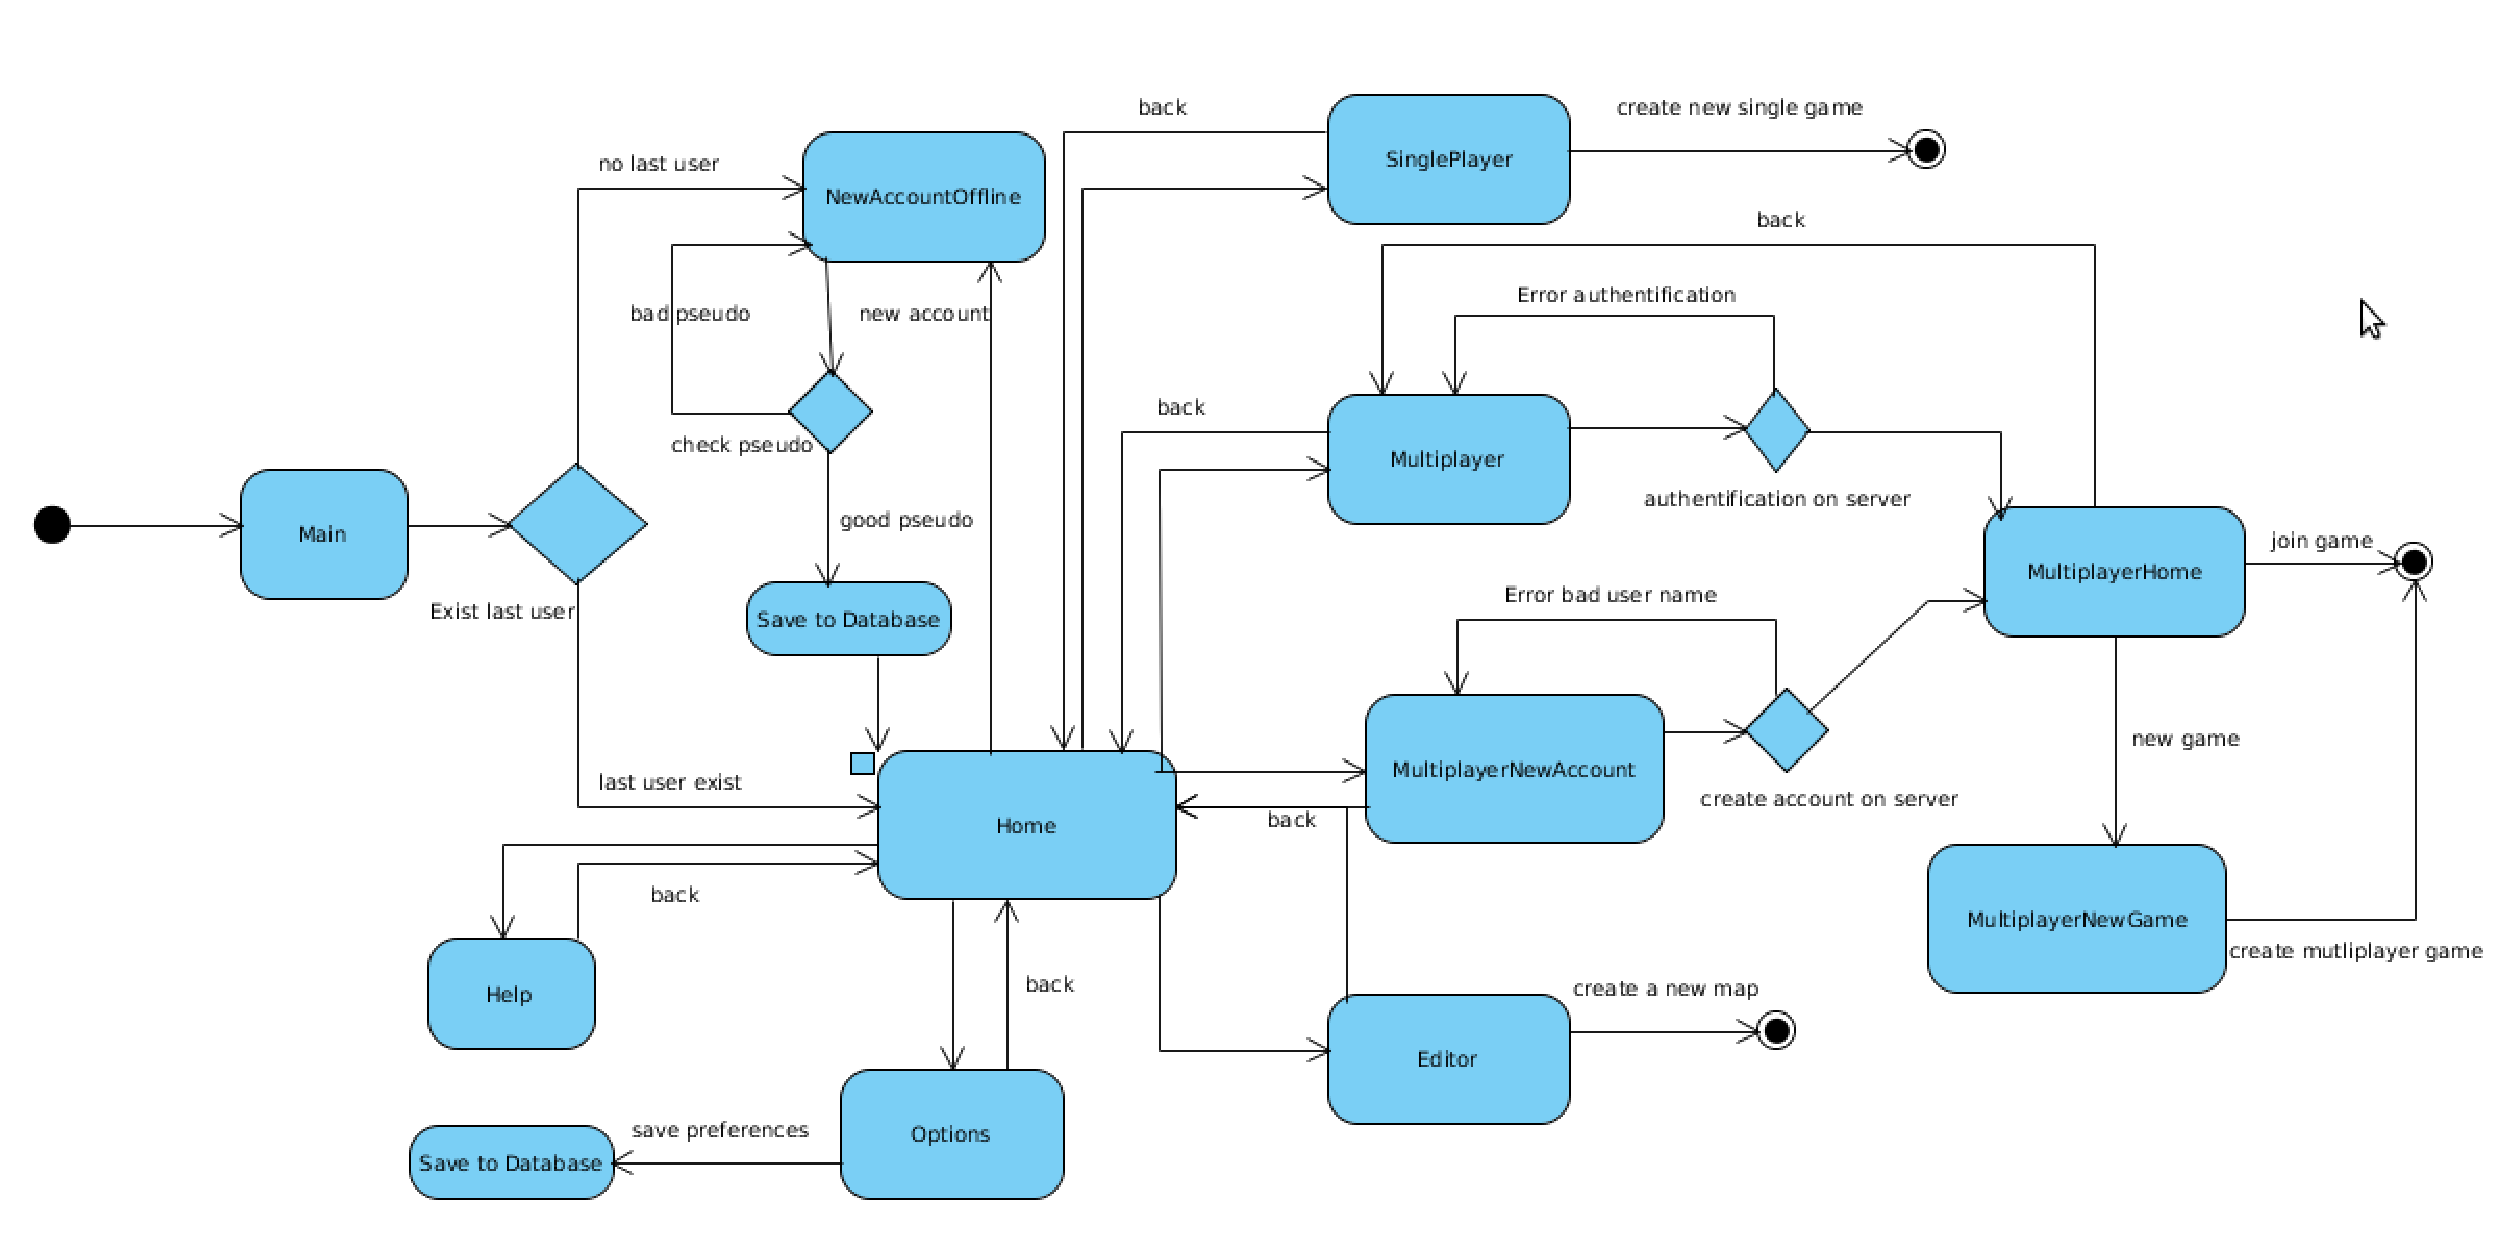
\includegraphics[width=23cm, angle=90]{Analyse/Img/diag_activity.eps}
		\caption{Diagramme d'activité}
	\end{figure}

	\paragraph{Base de données\\}
			
		Une base de données locale a elle aussi été conçue. Cette dernière a pour
		but de stocker plusieurs types de données.
				
		En effet dès lors qu'un compte local est crée sur le téléphone dans la
		table PlayerAccount, il est possible de conserver ses préférences de joueur
		tel que la couleur du joueur, le pseudonyme ou même ses paramètres de connexion multijoueur. 
		Vous pourrez créer autant de comptes locaux que vous le désirez, et il
		sera possible possible d'éditer ou choisir son compte.
				
		L'application est par ailleur en mesure de conserver
		les valeurs sonores, la langue et même le dernier utilisateur de
		l'application, grâce à un son id qui est clé étrangère dans la table System(lastUser).
				
		De plus l'application sera délivrée avec quelques cartes officielles, mais
		l'utilisateur aura libre droit de créer ses propres cartes de jeu via un
		éditeur. Elles seront alors stockées dans la table Map avec toujours une
		clé étrangère vers l'id de son créateur(owner). \\
		
		\newpage
				
		\begin{figure}
			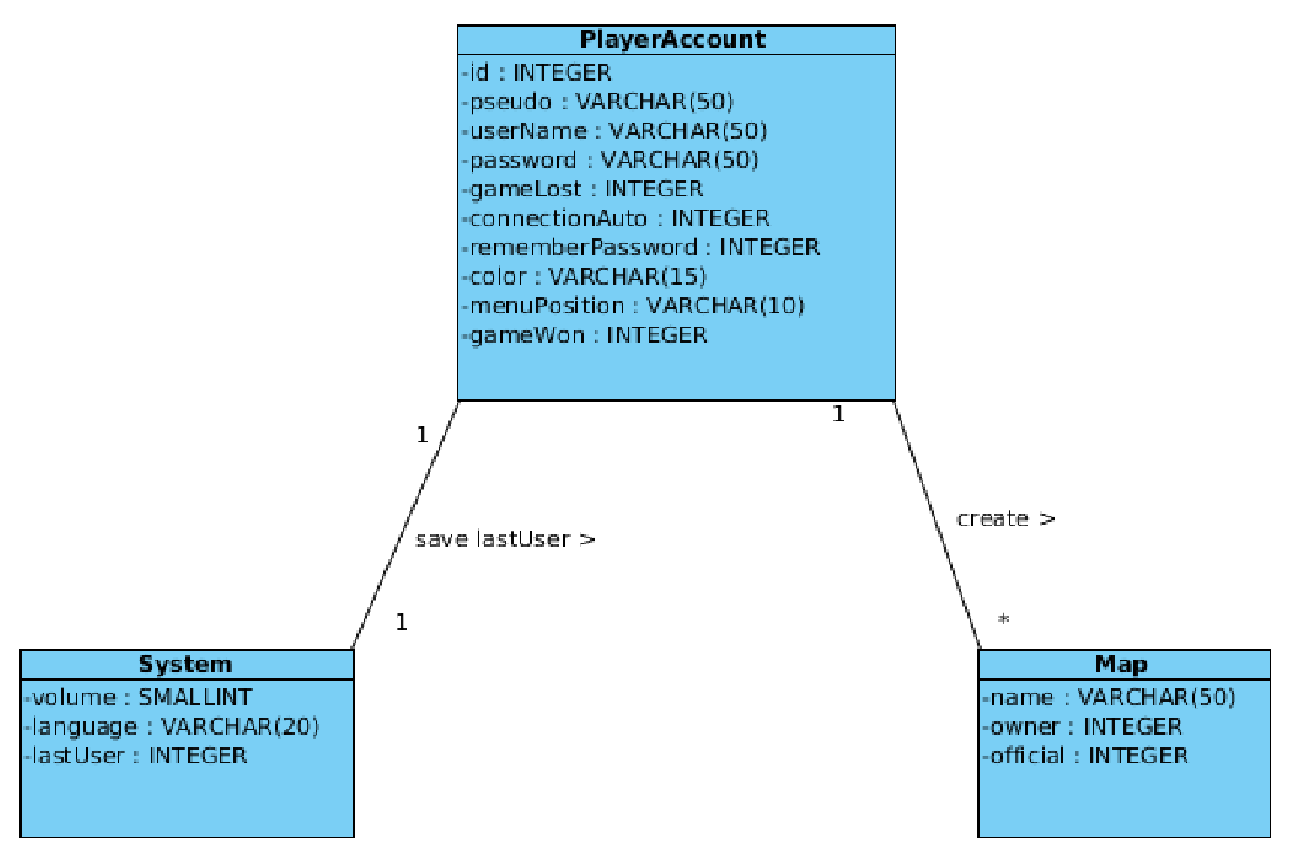
\includegraphics[width=11cm]{./Analyse/Img/menu_bdd.eps}
			\caption{Diagramme de classe Base de données}
		\end{figure}
		
		
		
						
	\paragraph{Scénarios}
	
	
\subsection{Editeur de carte}	

	L'éditeur de carte est une fonctionnalité qui va permettre à un utilisateur de créer facilement ses propres cartes pour ensuite y jouer dessus contre l'intéligence artificielle. Après avoir réfléchi sur toutes les fonctionnalités que l'éditeur de carte devait remplir, nous avons retenu celles-ci : permettre à l'utilisateur de créer une nouvelle carte, mais aussi de charger une ancienne carte précèdemment créée. Ensuite lui donner la possibilité de modifier le sol de la carte et aussi ajouter ou supprimer des blocs de la carte et enfin la dernière fonctionnalité que l'éditeur de carte implémente c'est de pouvoir placer les différents points de départ des joueurs sur la carte.
		
	Pour réaliser cette partie de l'application, nous avons utilisé le modèle de conception MVC pour diviser le code de l'éditeur de carte. Grâce a cette décomposition, le code est plus lisible et plus facile à réutiliser. 
			
	\subsubsection*{Modèle}
		La partie modèle va contenir toute les données de l'éditeur de carte. Les cartes sont les principales données qu'il va devoir manipuler. Pour cela nous avons décidé de la réprésenter sous la forme de deux matrices, la première représentant les objets du premier niveau (le sol) et la deusième la matrice du second niveau (les blocs, les points de départ des joueurs, etc).
			
			
	\subsubsection*{Vue}
		Ensuite, la vue représentera l'interface graphique de notre éditeur de carte. La principale difficulté pour réaliser l'interface graphique était de devoir rentrer toutes les informations nécessaires pour l'éditeur de carte dans un écran de type smartphone \footnote{Traduit littéralement comme \og téléphone intéligent \fg \, en français, c'est un terme utilisé pour désigner les téléphones évolués, qui possèdent des fonctions similaires à celles des assistants personnels. Certains peuvent lire des vidéos, des MP3 et se voir ajouter des programmes spécifiques.}. Après plusieurs prototypes d'interface, nous avons décide de séparer l'interface en trois parties. Tout d'abord la plus grande partie, l'affichage de la carte, qui comment étant la principale information à afficher, nous avons essayé de maximiser sa taille. Ensuite un menu à droite permettant au joueur de changer d'outil. Et la dernière partie affiche les différents éléments permettant de controler l'éditeur de carte. L'utilisateur aura juste à choisir l'outil qu'il veut placer sur la carte grâce au menu de droite et ensuite lui suffira d'appuier sur la carte pour placer un bloc dessus.
		
%		\begin{figure}
			\begin{center}
				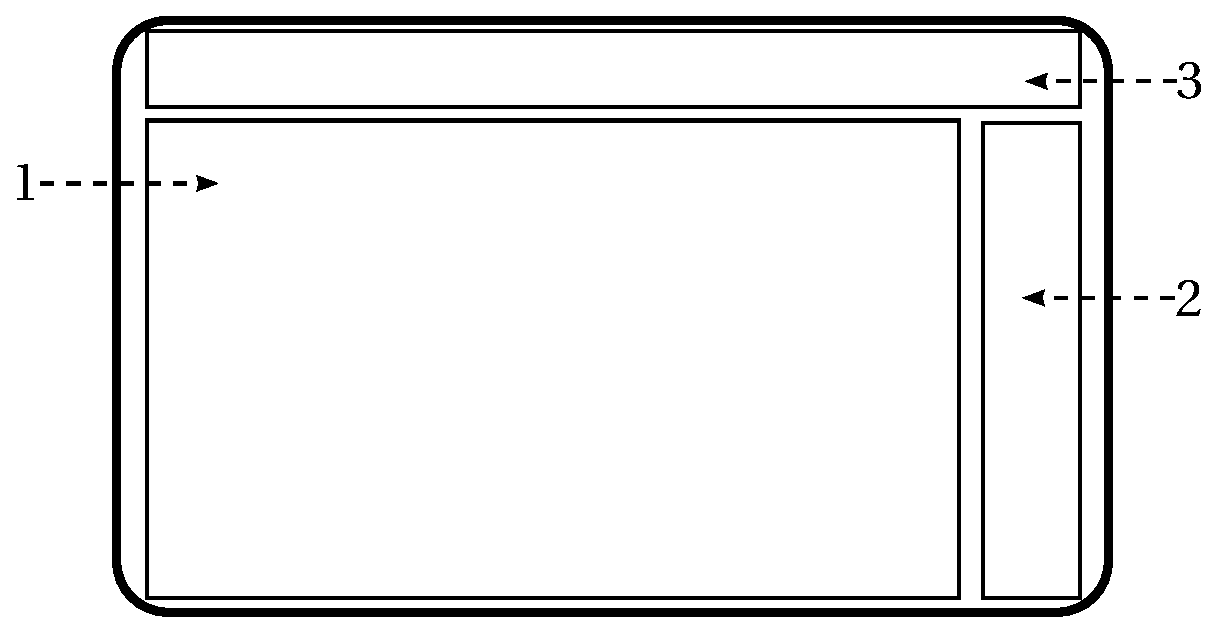
\includegraphics[width=11cm]{./Analyse/Img/14-Editeur_de_niveau.eps}
			\end{center} 
%		 	\caption{Poulpy est multicolore}
%		 	\label{Poulpy est multicolore}
%		\end{figure}
			
			
	\subsubsection*{Controleur}
		Pour finir le controleur aurra pour but de faire la liaison entre les données du modèle et de la vue. Chaque vue possède son controleur, et il y a un controleur gobal possédant les controleurs de chaque vue.
			

\subsection{Jeu}
	\begin{itemize}
		\item{Diagramme classe}
		\item{Gameplay}
		\item{Gestion images / tile mapping}
		\item{Images}
		\item{Sons}
	\end{itemize}
			

\subsection{Réseau}
		
	\paragraph{Serveur\\}
			
		Il a été fixé dans le cahier des charges que notre serveur devrait pouvoir
		effectuer plusieurs tâches particulières séparées. Nous avons donc décidé de
		les compartimenter en classes.
			
		Les six éléments situés sur la partie haute du schéma
		ci-dessous(respectivement Inscription, Connection, GamesList, CreateGame,
		ConnectionGame et ManageGame), réprésente les différents tâches demandées.
		Elles sont reliées à une classe nommée contexte, qui leur permettra d'accéder
		aux mêmes données sans qu'il y ait de conflits. La partie basse représente les
		objets qui seront utilisés pour les parties en multijoueurs. Bien évidemment
		ces objets sont très proches de ceux utilisés dans les parties
		locales(Schéma 3.1).
		
		Le scénarios le plus probable serait le suivant. Un utilisateur désire jouer
		en ligne contre de vrais joueurs. 
		Il va alors passer par l'inscription et créer son compte sur le
		serveur(Inscription). Une fois cette étape obligatoire faite, il pourra choisir entre rejoindre une partie en ligne
		en cour(ConnectionGame), ou en créer un nouvelle(CreateGame). Dès lors qu'il
		aura accès à une partie en ligne, un contact régulier avec le serveur sera
		obligatoire afin de réaliser les interactions entre les différents
		joueurs(ManageGame). Tout ceci devra se réaliser bien sûr dans une durée
		infime afin de ne pas pénaliser les joueurs.
		
	\paragraph{Base de données\\}
		Afin de pouvoir conserver les utilisateurs en ligne ainsi que leurs infos
		personnels et permettre une authentification, nous avons dû établir une
		base de données sur le serveur. Cette dernière à été pensé comme demandé pour 
		l'enregistrement de comptes. Une unique table nommée Users remplie donc cette
		fonction. Le serveur devra pouvoir y accéder en écriture(inscription) comme
		en lecture(connexion).
			
		Elle ne comportera que deux champs, userName et password. Dès lors que
		l'utilisateur désirera créer un compte multijoueur, il renseignera dans
		l'application son userName souhaité ainsi que son mot de passe. 
		Ce couple sera 	alors envoyé au serveur qui vérifiera dans cette base de
		données, que le userName(unique) n'est pas déjà utilisé. Auquel cas un nouveau n-uplet sera
		inséré et permettra l'authentification de l'utilisateur par la suite. Les mots
		de passe seront bien évidement crypté pour des raisons de sécurité.
			
		\begin{figure}
			\includegraphics[scale = 0.5]{Analyse/Img/serveur.eps}
			 \caption {Serveur}
		\end{figure}
		
		\newpage
		
	